% !TeX spellcheck = en_US
\section{Simulation of different vaccination strategies in girls and boys with the aim to eradicate the HPV oncogenic HR}\label{vaccinationStrategies}
In this Chapter, we are going to simulate the scenarios where we vaccinate GARDASIL9 to boys and girls with a coverage of $60\%$, $75\%$ and $90\%$. Then, we will see when a decline of $65\%$, $75\%$, $85\%$ and $95\%$ is reached in all the cases for HPV oncogenic HR. Our results will be compared with the ones in \cite{Brisson2016}, where the authors consider that the elimination of the HPV HR included in GARDASIL9 (the oncogenic ones) will be reached after $80$ years vaccinating boys and girls with a coverage of $80\%$. The results can be seen in Table \ref{tabla:decline_HR_onco}.

\begin{table}[!h]
	\hspace*{-6em}%me lo saco de la manga de Internet
	\centering
	\small
	\begin{tabular}{c|lll}
        \\
        \hline
        \multicolumn{4}{c}{\textbf{Vaccination of boys and girls with a coverage of $60\%$}}\\
        \hline
        Decline & Women &  Men & MSM \\ 
        \hline		
$ 65 \%$ & year 2040, CI95\% $[ 2029 , 2051 ]$ & year  2047, CI95\% $[ 2031 , 2053 ]$ & year $-$, CI95\% $[ 2053, - ]$ \\
$ 75 \%$ & year 2050, CI95\% $[ 2032 , 2055 ]$ & year  2058, CI95\% $[ 2038, 2070 ]$ & year  $-$, CI95\% $[ - , - ]$ \\
$ 85 \%$ & year 2084, CI95\% $[ 2069, - ]$ & year  $-$, CI95\% $[ - , - ]$ & year  $-$, CI95\% $[ - , - ]$ \\
$ 95 \%$ & year $-$, CI95\% $[ - , - ]$ & year  $-$, CI95\% $[ - , - ]$ & year  $-$, CI95\% $[ - , - ]$ \\
		\\
		\hline 		
		\multicolumn{4}{c}{\textbf{Vaccination of boys and girls with a coverage of $75\%$}}\\
		\hline
		Decline & Women &  Men & MSM \\ 
		\hline 
$ 65 \%$ & year 2034, CI95\% $[ 2028 , 2047 ]$ & year 2039, CI95\% $[ 2028 , 2048 ]$ & year 2045, CI95\% $[ 2042 , 2049 ]$ \\
$ 75 \%$ & year 2042, CI95\% $[ 2030 , 2050 ]$ & year 2046, CI95\% $[ 2032 , 2052 ]$ & year 2053, CI95\% $[ 2049 , 2059 ]$ \\
$ 85 \%$ & year 2050, CI95\% $[ 2033 , 2054 ]$ & year 2054, CI95\% $[ 2042 , 2056 ]$ & year $-$, CI95\% $[ - , - ]$ \\
$ 95 \%$ & year $-$, CI95\% $[ 2060 , - ]$ & year $-$, CI95\% $[ - , - ]$ & year $-$, CI95\% $[ - , - ]$ \\
         \\
         \hline
         \multicolumn{4}{c}{\textbf{Vaccination of boys and girls with a coverage of $90\%$}}\\
         \hline
         Decline & Women &  Men & MSM \\ 
         \hline
$ 65 \%$ & year 2032, CI95\% $[ 2027 , 2046 ]$ & year 2035, CI95\% $[ 2027 , 2046 ]$ & year 2039, CI95\% $[ 2036 , 2042 ]$ \\
$ 75 \%$ & year 2038, CI95\% $[ 2029 , 2050 ]$ & year 2041, CI95\% $[ 2030 , 2049 ]$ & year 2044, CI95\% $[ 2041 , 2047 ]$ \\
$ 85 \%$ & year 2046, CI95\% $[ 2032 , 2052 ]$ & year 2048, CI95\% $[ 2033 , 2052 ]$ & year 2050, CI95\% $[ 2047 , 2052 ]$ \\
$ 95 \%$ & year 2054, CI95\% $[ 2042 , 2056 ]$ & year 2055, CI95\% $[ 2048 , 2057 ]$ & year $-$, CI95\% $[ 2056 , - ]$
	\end{tabular} 
	\caption{Here, we show when a decline of HPV oncogenic HR of $65\%$, $75\%$, $85\%$ and $95\%$ is reached when vaccinating boys and girls with a coverage of $60\%$, $75\%$ and $90\%$. MSM are included in men, and also considered separately.}
	\label{tabla:decline_HR_onco}
\end{table}

Now, in Figure \ref{fig:erradicacion}, we show some graphs about the decline of HPV oncogenic in 14-64 years old women, men and MSM with coverage for women and men of $75\%$ and $90\%$. The difference between the percentage of vaccinated individuals (yellow lines) and the decline of the HPV (cyan lines) is a measure of the herd immunity effect on each population. As we can see, the herd immunity effect on women and men are similar. The small differences are because men include MSM even though the percentage of MSM is low respect to the total of men. Nevertheless, in MSM, the herd immunity is low, because their high number of LSP that MSM have.  

\begin{figure}[!]
	\centering
	\begin{tabular}{cc}
		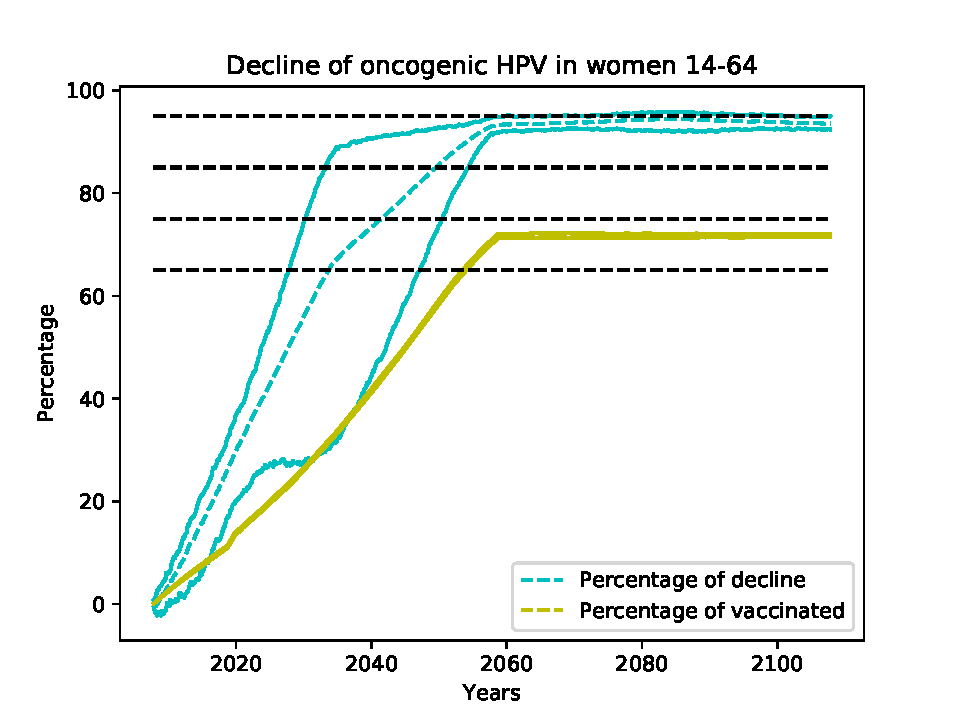
\includegraphics[width=0.5\linewidth]{IMGs/9.-Erradicacion_ONCO/onco_muj_75.pdf}	& 
		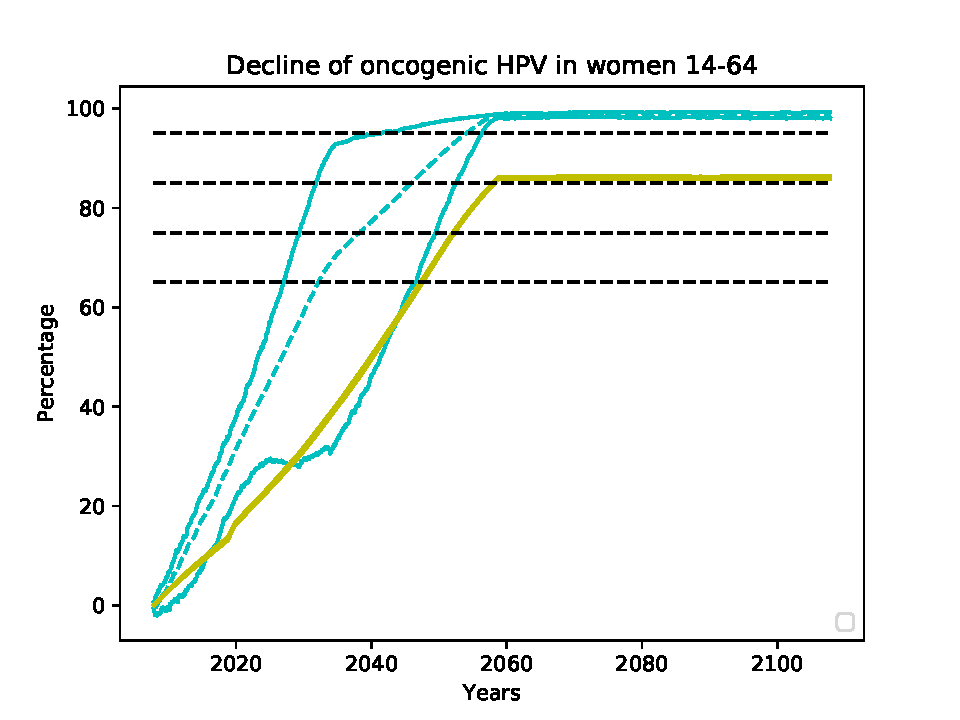
\includegraphics[width=0.5\linewidth]{IMGs/9.-Erradicacion_ONCO/onco_muj_90.pdf}  \\ 
		Decline. Women. Coverage $75\%$	& Decline. Women. Coverage $90\%$ \\ 
		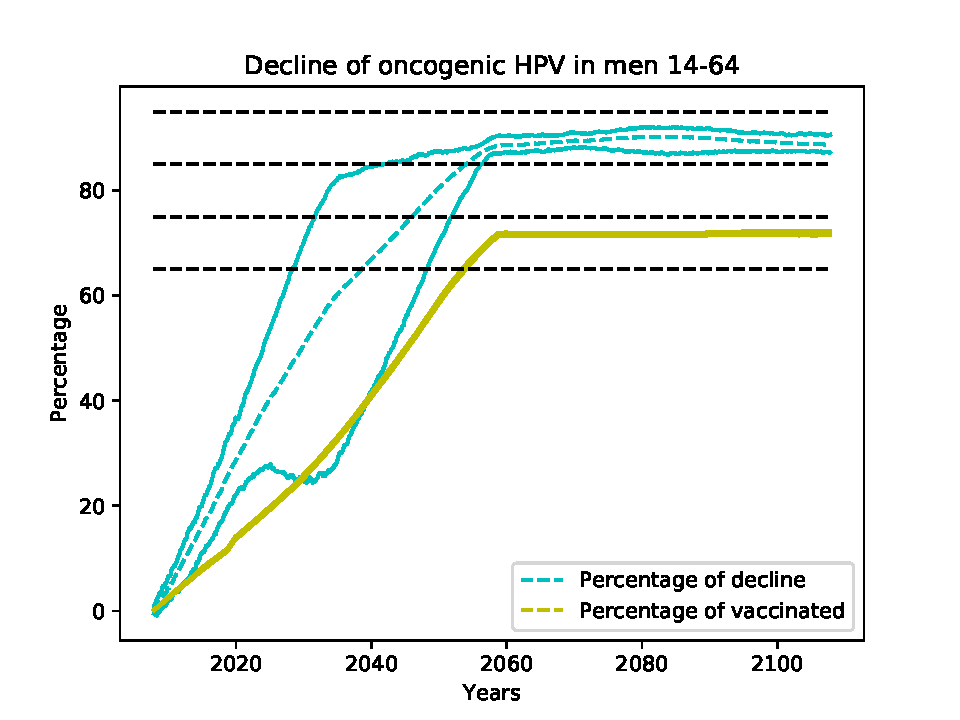
\includegraphics[width=0.5\linewidth]{IMGs/9.-Erradicacion_ONCO/onco_hom_75.pdf}	& 
		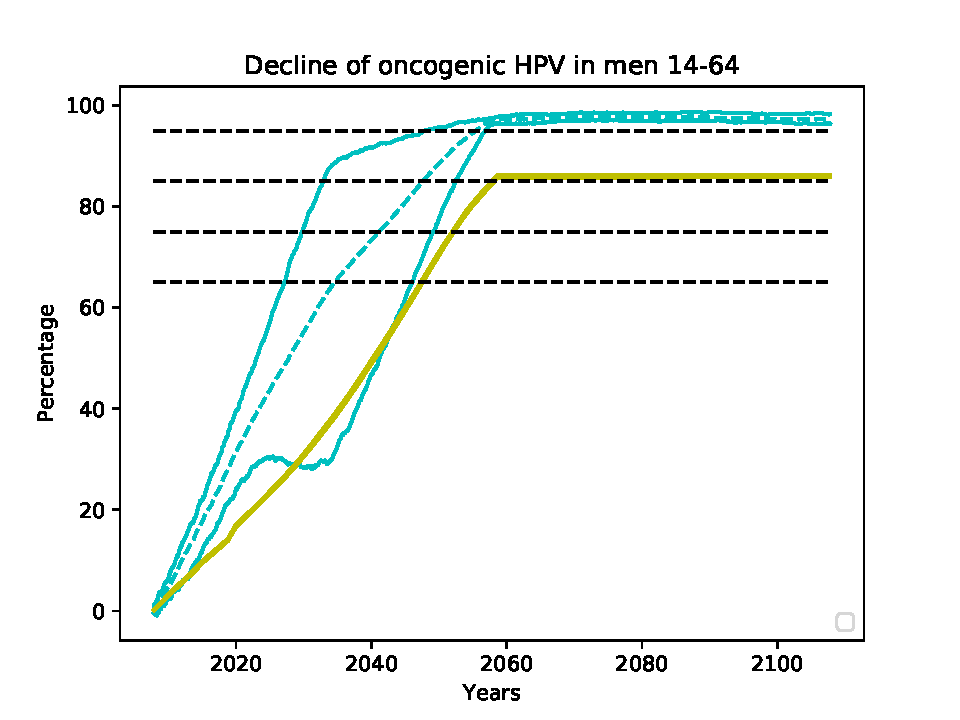
\includegraphics[width=0.5\linewidth]{IMGs/9.-Erradicacion_ONCO/onco_hom_90.pdf}  \\ 
		Decline. Men. Coverage $75\%$	& Decline. Men. Coverage $90\%$ \\ 		
		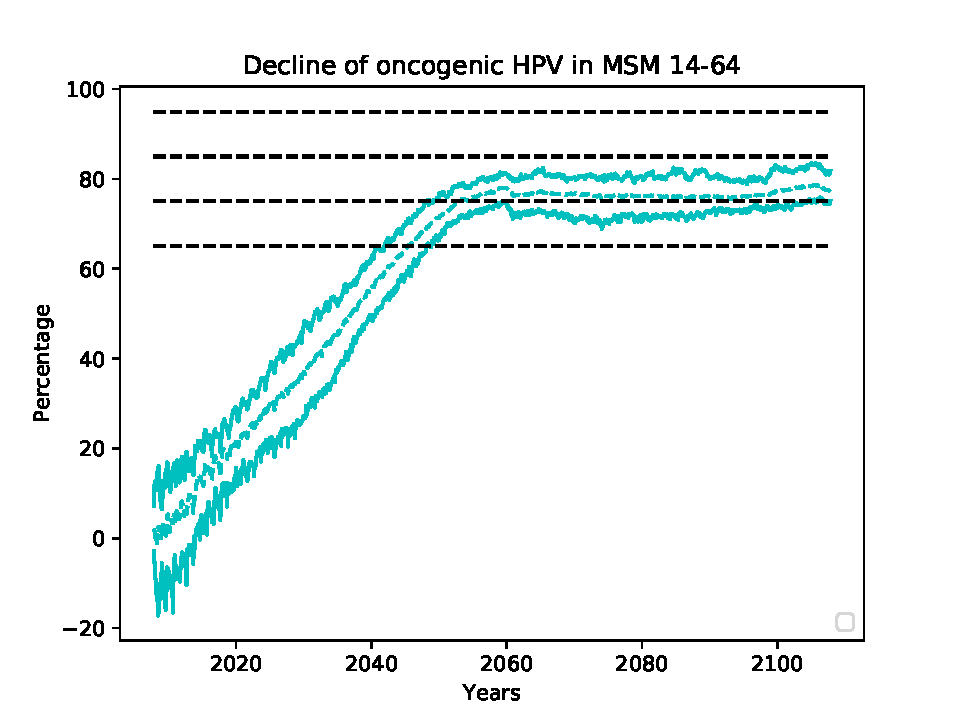
\includegraphics[width=0.5\linewidth]{IMGs/9.-Erradicacion_ONCO/onco_MSM_75.pdf}	& 
		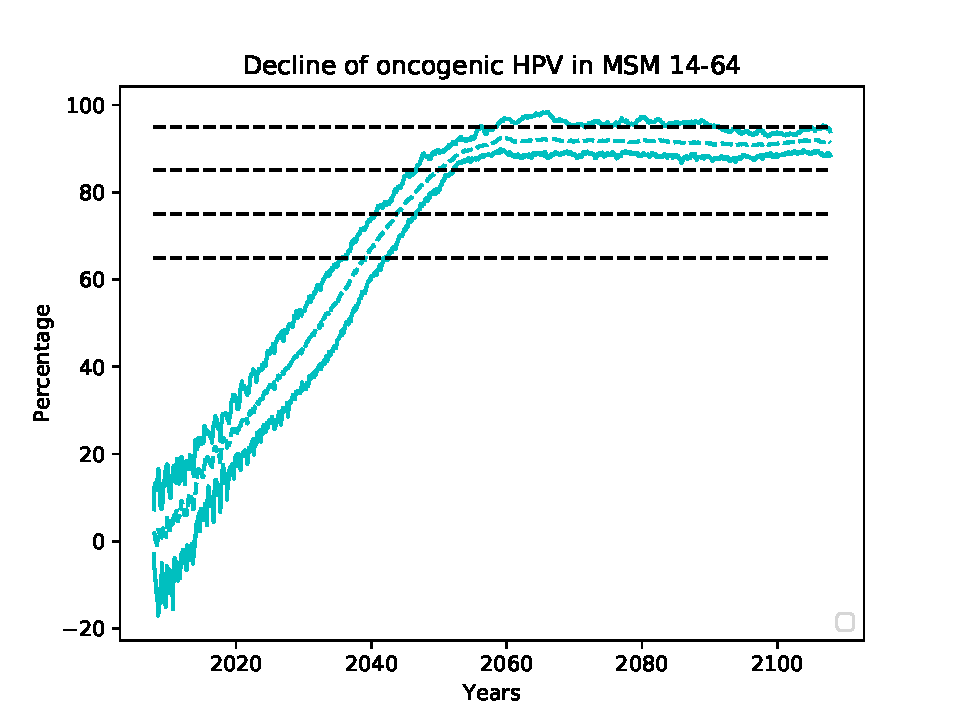
\includegraphics[width=0.5\linewidth]{IMGs/9.-Erradicacion_ONCO/onco_MSM_90.pdf}  \\ 
		Decline. MSM. Coverage $75\%$	& Decline. MSM. Coverage $90\%$
	\end{tabular} 
	\caption{Decline of HPV oncogenic in 14-64 years old women, men and MSM with coverage for women and men of $75\%$ and $90\%$ over the time. The horizontal dashed lines point out the decline percentages of $65\%$, $75\%$, $85\%$ and $95\%$. The difference between the cyan and the yellow lines is a measure of the herd immunity effect on each population. In this case, due to the high coverage, we can see herd immunity effect in MSM in the long-run.}
	\label{fig:erradicacion}
\end{figure}

As we can see in the Figure \ref{fig:erradicacion}, the highest values of decline are reached around $2060$ in all the graphs, that is, after a complete generation has been vaccinated. Therefore, a high coverage for women and men during a whole generation has to be considered if we want to eradicate the cancer produced by HPV oncogenic. 

Nevertheless, Figure \ref{fig:erradicacion} shows that the variation of the decline in the long-run between the vaccination of $75\%$ to $90\%$ is small if we think that we need an increase of $15\%$ in coverage. In average, the difference is $7.5\% - 8.7\%$ in the decline for men, $13.1\%-16\%$ in the decline for MSM and $4.3\%-5.2\%$ in the decline for women. This fact may suggest that, reaching coverages around $70\% - 75\%$ is enough to have a high protection in the whole population without a significant increasing of the vaccination cost to achieve small increases in the decline in the long-run.

Also, we would like to point out that the herd immunity effect, measured by the difference between the decline lines (cyan) and the vaccination lines (yellow), is similar in men and women, and there is a small herd immunity in MSM in the long-run, due to the high vaccine coverage.

In recent papers as \cite{Brisson2016, SIMMS2019394, BRISSON2019319}, the authors find possible the elimination of the oncogenic HPV included in GARDASIL9 in around a generation. However, our model with its accurate replication of the herd immunity effect, suggests that we have to be cautious. MSM have small herd immunity effect and, therefore, if we are not able to vaccinate almost all the MSM with higher coverages on them, the unprotected MSM may preserve the circulation of the virus due to their high number of sexual partners. 

  